\chapter{Testing}
\label{cap:testing}
\begin{center}
    \begin{figure}
        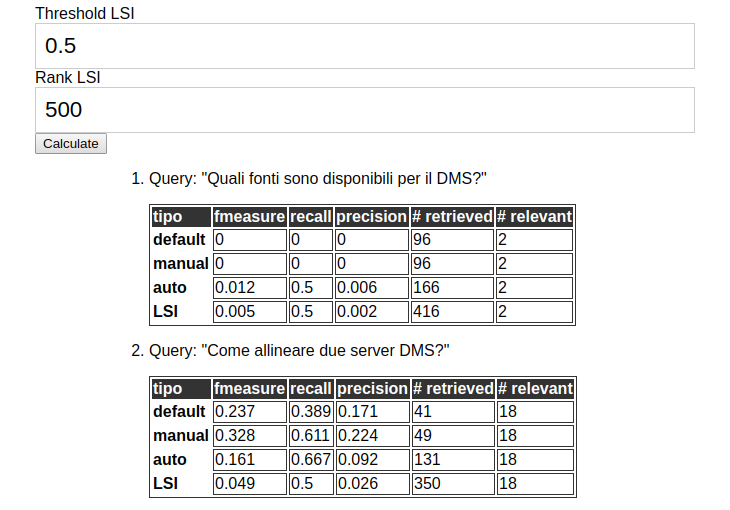
\includegraphics[scale=0.5]{immagini/ir_eval.png}
        \caption{Esempio di risultato dei test}
     \end{figure}
\end{center}
    
    
    Parte del lavoro dello stage è stato realizzare una collezione di test che permettessero di valutare la ricerca. Era quindi richiesto, costruire la cosiddetta ground truth, ovvero:
    \begin{itemize}
        \item individuare, per ogni ricerca, quali fossero i documenti pertinenti;
        \item le ricerche dovevano contenere falsi negativi;
        \item le ricerche dovevano essere frasali (e non con un paio di termini).
    \end{itemize}

    Viste le dimensioni del corpus e i vincoli precedentemente elencati, sono riuscito ad individuare 20 ricerche con falsi negativi. Un paio di esempi di test è disponibile in §\ref{cap:esempi-test}.
    \section{Metriche}
    Le metriche (f-measure, precision e recall) sono state scelte dall'azienda prima dell'inizio dello stage e sono state presentate in §\ref{sub:metriche-valutazione}.

    \section{Risultati}
    È risultato evidente dai test che la soluzione naive, basata sull'uso di un tesauro manualmente costruito, sia stata quella che ha avuto il miglior risultato: questo probabilmente deriva dal fatto che il corpus era piccolo nel complesso e i documenti erano anch'essi piccoli. (i frammenti audio estratti dal servizio di trascrizione) Nella pagina dei risultati dei test è possibile modificare i parametri di soglia e rango della matrice,  senza dover ricalcolare la decomposizione (che è onerosa in termini di tempo).

    \FloatBarrier